\documentclass[notheorems,aspectratio=169]{beamer}

\author{Владислав Шаршуков\\\vspace{8mm}Научный руководитель: Чижова О.~Н.}
\date{\today}
\title{Построение динамического регулятора для стабилизации линейных стационарных систем}

%% \usetheme{Warsaw}
\usetheme{default}
\usefonttheme{serif}

\usepackage[utf8]{inputenc}
\usepackage[T2A]{fontenc}
\usepackage[russian]{babel}
\usepackage{graphicx}
\usepackage{longtable}
\usepackage{wrapfig}
\usepackage{rotating}
\usepackage{physics}
\usepackage[normalem]{ulem}
\usepackage[makeroom]{cancel}
\usepackage{amsmath}
\usepackage{amssymb}
\usepackage{capt-of}
\usepackage{hyperref}

\usepackage[backend=biber]{biblatex}

\graphicspath{ {./Images/} }

\addbibresource{DynamicRegulatorPresentation.bib}

\theoremstyle{definition}
\newtheorem{theorem}{Теорема}
\newtheorem{definition}{Определение}
\newtheorem{remark}{Замечание}
\newtheorem{proposition}{Утверждение}
\newtheorem{lemma}[theorem]{Лемма}
\newtheorem{corollary}[theorem]{Следствие}
\newtheorem{solution}{Решение} % FIXME: solution is not a theorem

\newcommand{\highlight}[1]{{\color{red} #1}}
%% \newcommand{\abs}[1]{\left| #1 \right|}

\newcommand{\paren}[1]{\left(#1\right)}
\renewcommand{\emph}[1]{\uline{#1}}
\renewcommand{\Re}{\operatorname{Re}}
\renewcommand{\Im}{\operatorname{Im}}

\setbeamertemplate{section in toc}[sections numbered]
\setbeamertemplate{footline}{}
\setbeamertemplate{headline}{}
\setbeamertemplate{navigation symbols}{}

%% ================================== %%

\begin{document}

\begin{frame}
  \titlepage{}
\end{frame}

\begin{frame}{Линейная система}
  Рассмотрим линейную стационарную систему
  \begin{equation*}
    \begin{aligned}
      \dot{\vb{x}}(t) &= A \vb{x}(t) + B \vb{u}(t) \\
      \vb{y}(t) &= C \vb{x}(t),
    \end{aligned}
  \end{equation*}

  \begin{itemize}
  \item $\vb{x}(t): \mathbb{R} \to \mathbb{R}^n$ --- неизмеряемое состояние
  \item $\vb{u}(t): \mathbb{R} \to \mathbb{R}^m$ --- управление
  \item $\vb{y}(t): \mathbb{R} \to \mathbb{R}^p$ --- выход системы
  \item $A \in \mathbb{R}^{n \times n}$, $B \in \mathbb{R}^{n \times m}$, $C \in \mathbb{R}^{p \times n}$.
  \end{itemize}
\end{frame}

\begin{frame}{Постановка задачи}
  \begin{itemize}
  \item Полностью управляемой стационарной системе с помощью обратной связи
    вида $\vb{u}(t) = -K\hat{\vb{x}}(t)$ можно придать произвольные динамические
    свойства.~\cite{Andreev1976}

  \item Для полностью наблюдаемой системы можно построить асимптотический идентификатор.~\cite{Andreev1976,Smirnov2022}
  \end{itemize}

  Требуется построить динамический регулятор, обеспечивающий асимптотическую устойчивость замкнутой системе.

  \begin{center}
    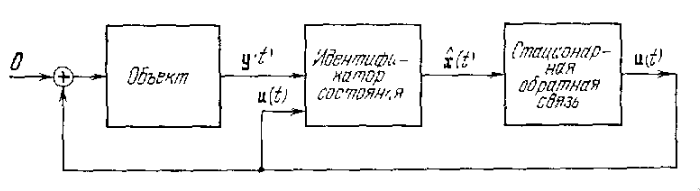
\includegraphics[width=12cm]{Regulator}
  \end{center}
\end{frame}

\begin{frame}{Использование идентификатора полного порядка}
  Дано:
  \begin{itemize}
  \item Система $\{A, B, C\}$ полностью управляемая и полностью наблюдаемая;
  \item Идентификатор состояния полного порядка
    \begin{equation*}
      \dot{\hat{\vb{x}}}(t) = \left[A - LC\right] \hat{\vb{x}}(t) + L \vb{y}(t) + B \vb{u}(t),
    \end{equation*}
    причём $p_{\left[A - LC\right]}(\lambda) = \varphi_{\text{и}}(\lambda)$;
  \item Обратная связь $\vb{u}(t) = -K\hat{\vb{x}}(t)$,
    причём $p_{\left[A - BK\right]}(\lambda) = \varphi_{\text{у}}(\lambda)$.
  \end{itemize}
  
  Тогда характеристический полином замкнутой системы $2n$-го порядка
  \begin{equation*}
    \begin{aligned}
      \dot{\vb{x}}(t) &= A \vb{x}(t) - BK \hat{\vb{x}}(t), \\
      \dot{\hat{\vb{x}}}(t) &= \left[A - LC\right] \hat{\vb{x}}(t)
      + LC \vb{x}(t) - BK \hat{\vb{x}}(t)
    \end{aligned}
  \end{equation*}
  совпадает с произведением выбранных полиномов: $\varphi_{\text{з}}(\lambda) = \varphi_{\text{у}}(\lambda) \cdot \varphi_{\text{и}}(\lambda)$.
\end{frame}

\begin{frame}{Доказательство}
  Перепишем замкнутую систему в виде
  \begin{equation*}
    \left[%
      \begin{array}{c}
        \dot{\vb{x}} \\
        \dot{\hat{\vb{x}}}
      \end{array}
      \right]
    =
    \left[
      \begin{array}{cc}
        A & -BK \\
        LC & A - LC - BK
      \end{array}
      \right]
    \left[
      \begin{array}{c}
        \vb{x} \\
        \hat{\vb{x}}
      \end{array}
      \right]
  \end{equation*}

  Сделаем невырожденную замену переменной $\tilde{\vb{x}}(t) = \vb{x}(t) - \hat{\vb{x}}(t)$; матрица
  этого преобразования имеет вид
  \begin{equation*}
    \left[
      \begin{array}{cc}
        E_{n \times n} & 0_{n \times n} \\
        E_{n \times n} & E_{n \times n}
      \end{array}
      \right].
  \end{equation*}

  В новых координатах матрица система примет вид
  \begin{equation*}
    \left[
      \begin{array}{c}
        \dot{\vb{x}} \\
        \dot{\tilde{\vb{x}}}
      \end{array}
      \right]
    =
    \left[
      \begin{array}{cc}
        A - BK & \ast \\
        0_{n \times n} & A - LC
      \end{array}
      \right]
    \left[
      \begin{array}{c}
        \vb{x} \\
        \tilde{\vb{x}}
      \end{array}
      \right].
  \end{equation*}

  Характеристический полином блочно-диагональной матрицы этой системы: $\varphi_{\text{з}}(\lambda) = \varphi_{\text{у}}(\lambda) \cdot \varphi_{\text{и}}(\lambda)$. $\quad \square$
\end{frame}

\begin{frame}{Применение идентификаторов неполного порядка ($p=1$)}
  Дано:
  \begin{itemize}
  \item Система $\{A, B, c\}$ полностью управляемая и полностью наблюдаемая;
  \item Идентификатор состояния порядка $(n-1)$
    \begin{equation*}
      \dot{\hat{\vb{x}}}_1(t) = \bar{A} \hat{\vb{x}}_1(t) + \bar{\vb{a}}_n y(t) + B_1 \vb{u}(t), \qquad \hat{\vb{x}}_1(t): \mathbb{R} \to \mathbb{R}^{(n-1)}
    \end{equation*}
    с заданным многочленом $p_{\bar{A}}(\lambda) = \varphi_{\text{и}}(\lambda)$~\cite{Andreev1976};
  \item Обратная связь $\vb{u}(t) = -K\hat{\vb{x}}(t), \; p_{\left[A - BK\right]}(\lambda) = \varphi_{\text{у}}(\lambda)$.
  \end{itemize}
  
  Тогда характеристический полином замкнутой системы $(2n-1)$-го порядка
  совпадает с произведением выбранных полиномов: $\varphi_{\text{з}}(\lambda) = \varphi_{\text{у}}(\lambda) \cdot \varphi_{\text{и}}(\lambda)$.
\end{frame}

\begin{frame}{Доказательство}
  Замкнутая система имеет вид
  \begin{equation*}
    \begin{aligned}
      \dot{\vb{x}}(t) &= A \vb{x}(t) - BK \hat{\vb{x}}(t), \\
      \dot{\hat{\vb{x}}}_1(t) &= \overline{A} \hat{\vb{x}}_1(t) + \bar{\vb{a}}_n \hat{x}_n(t) - B_1 K \hat{\vb{x}}(t).
    \end{aligned}
  \end{equation*}
  где
  \begin{equation*}
    \hat{\vb{x}}(t) =
    \left[
      \begin{array}{c}
        \hat{\vb{x}}_1(t) \\
        \hat{x}_n(t)
      \end{array}
      \right], \qquad \hat{\vb{x}}(t): \mathbb{R} \to \mathbb{R}^n.
  \end{equation*}
  Проведём замену переменных $\tilde{\vb{x}}(t) = \hat{\vb{x}}_1(t) - \bar{\vb{x}}(t)$:
  \begin{equation*}
    \left[
      \begin{array}{c}
        \dot{\vb{x}} \\
        \dot{\tilde{\vb{x}}}
      \end{array}
      \right]
    =
    \left[
      \begin{array}{cc}
        A - BK & \ast \\
        0_{(n-1) \times n} & \bar{A}
      \end{array}
      \right]
    \left[
      \begin{array}{c}
        \vb{x} \\
        \tilde{\vb{x}}
      \end{array}
      \right].
  \end{equation*}
  Матрица этой системы клеточно-диагональная, поэтому характеристический многочлен этой системы представим в виде
  $\varphi_{\text{з}}(\lambda) = \varphi_{\text{у}}(\lambda) \cdot \varphi_{\text{и}}(\lambda)$. $\quad \square$
\end{frame}

\begin{frame}{Применение идентификаторов неполного порядка ($p \leqslant n$)}
  Если $\vb{y}(t) : \mathbb{R} \to \mathbb{R}^p$, где $p \neq 0$, то
  систему $\{A, B, C\}$ можно представить как прямую сумму подсистем, для каждой из
  которых выход скалярный~\cite{Andreev1976}, поэтому справедлива
  \begin{theorem}
    Для полностью управлемой и полностью наблюдаемой линейной системы $\{A, B, C\}$ можно построить цепь
    обратной связи $(n-p)$--го порядка такую, что характеристический полином замкнутой системы
    $(2n-p)$--го порядка совпадает с заранее заданным вещественным полиномом.
  \end{theorem}
\end{frame}

\begin{frame}{Перспективы}
  Обощение результатов на:
  \begin{itemize}
    \item системы с $p$ зависимыми выходами;
    \item системы, подверженные помехам и внешним возмущениям;
    \item системы с запаздыванием.
  \end{itemize}
\end{frame}

\begin{frame}{Литература}
  \nocite{Andreev1976}
  \nocite{Kalman2004}
  \nocite{Polyak2019}
  \nocite{Smirnov2022}

  \printbibliography{}
\end{frame}

\end{document}
